 \documentclass[12pt]{article}
\usepackage[a4paper,  total={170mm,257mm},
 left=7mm,
 right=7mm,
 top=5mm,
 bottom=17mm
]{geometry}

\usepackage{array}
\usepackage{graphicx, subfig, wrapfig, fancyhdr, lastpage,makecell }
\newcommand\headerMe[2]{\noindent{}#1\hfill#2}
\usepackage[mathscr]{euscript}



\pagestyle{fancy}
\fancyhf{}

\cfoot{\em{Page \thepage \hspace{1pt} / \pageref{LastPage}}}
\begin{document}

\headerMe{Royaume du Maroc}{année scolaire \emph{2022-2023}}\\
\headerMe{Ministère de l'Éducation nationale, }{  Professeur :\emph{Zakaria Haouzan}}\\
\headerMe{du Préscolaire et des Sports}{Établissement : \emph{Lycée SKHOR qualifiant}}\\

\begin{center}

Devoir  N°4 - Semestre 02 \\
   Filière Tronc Commun Scientifique\\
Durée 3h00
\\
\hrulefill
\Large{Chimie 7pts - 63min}
\hrulefill\\

    \emph{Les  parties sont indépendantes}
\end{center}
%end Headerss------------------------
 
    
\section*{Partie 1 :Outils de description d'un système chimique. \dotfill (4pts) }
	L’oxyde d’azote $N_2O$ est utilisé comme gaz anesthésiant en chirurgie ou comme propulseur dans les bombes
	aérosol. Le volume molaire gazeux vaut $24,0 L.mol^{-1}$.

	\begin{enumerate}
		\item  Quelle est la masse molaire de l’oxyde d’azote ? \dotfill(0,25pts)
		\item Quelle quantité de matière contient un volume $V = 250,0 mL$ de ce gaz. Déduire le nombre des molécules d’oxyde d’azote. \dotfill (0,75pt)
		\item Calculer la masse de 50,0 mL de ce gaz. \dotfill (0,25pts)
\end{enumerate}

La phénolphtaléine est un indicateur coloré acido-basique de formule $C_{20}H_{14}O_4$ Elle est utilisée en solution
dans l’éthanol à la concentration $C=1,5.10^{-3}mol.L^{-1}$

\begin{enumerate}
	\item[4.] Quel est le solvant et le soluté de cette solution ? \dotfill(0,25pt)
	\item[5.]Quelle quantité de matière de phénolphtaléine doit être utilisée pour préparer 250mL de cette solution
alcoolique ?\dotfill (0,75pt)
\item[6.] Quelle est la masse de phénolphtaléine correspondante ? \dotfill (0,75pt)
\item[7.] On dispose d’une solution aqueuse $S_0$ de diiode de concentration $C_0 = 2,0.10^{-2} mol.L^{-1}$. On souhaite préparer un volume $V_1 = 250 mL$ de solution de diiode de concentration $C_1 = 4.10^{-3} mol.L^{-1}$

Déterminer le volume $V_0$ de solution $S_0$ de diiode qu’on doit prélever. Puis déterminer le facteur de dilution. \dotfill(1pt)

\end{enumerate}

\textbf{On donne en $g.mol^{-1}$:  }  $M(C)=12g.mol^{-1}$, $M(H)=1g.mol^{-1}$, $M(O)=16 g.mol^{-1}$ 

$M(N)=14 g.mol^{-1}$ et $N_A=6,02.10^{23}mol^{-1}$


%\begin{center}
%\begin{tabular}{ | c | c | c | }
	%\hline
	%\textbf{Espèce chimique }& \textbf{test} & \textbf{résultat} \\\hline 
 %Présence d’eau $H_2O$ & Sulfate de cuivre anhydre & ....................... \\\hline  
 %acide & ............. & ........................\\\hline 
%\end{tabular}
%\end{center}


%\begin{wrapfigure}[10]{r}{0.32\textwidth}
	%\vspace{-1.4cm}
	%\begin{center}
    %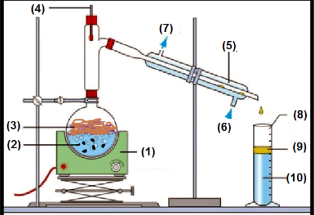
\includegraphics[width=0.32\textwidth]{./img/hydro.png}
	%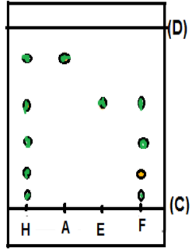
\includegraphics[width=0.2\textwidth]{./img/CCM.png}
%\end{center}
%\end{wrapfigure}

\section*{Partie 2 :Transformation chimique d’un système.\dotfill (3pts) }
%__________________Chimie ______________________-
%%%%%%%+_+_+_+_+_+_+_+_+_Partie1
On introduit un morceau d’aluminium $Al_{(S)}$ de masse $m=16,2g$ dans une solution d’acide chlorhydrique $(H^+_{(aq)}+Cl^-_{(aq)})$ de concentration   $C$=$0,24 mol/L$ et de volume $V=1L$. la réaction chimique mise en jeu entre le morceau d’aluminium $Al_{(S)}$ et les ions $H^+_{(aq)}$ produit les ions $Al^{3+}_{(aq)}$ et le dihydrogène gazeux $H_{2(g)}$.

\begin{enumerate}
	\item  Calculer $n_1$ et $n_2$ les quantités de matières initiales respectives de $H^+_{(aq)}$ et de $Al_{(S)}$.\dotfill (0,5pts)

	\item  Ecrire l’équation de la réaction mise en jeu équilibrée puis tracer le tableau d’avancement associé à cette
réaction. \dotfill (0,5pts)
\item  Déterminer $X_{max}$ l’avancement maximal puis déduire le réactif limitant. \dotfill(0,5pts)
\item  En se basant sur le tableau d’avancement , donner le bilan de matière à l’état final .\dotfill(0,5pts)
\item  déduire $V_{f(H_2)}$ le volume finale du dihydrogène produit à l’état final.\dotfill(1pt)
\end{enumerate}

\textbf{Données : }La masses molaires $M(Al) = 27g/mol$ et Volume molaire $V_m = 24 L.mol^{-1}$.


%_____________________________________PHYSIque Partie 22222____________________________________________________________________________
\begin{center}
    \vspace{0.5cm}
\hrulefill
\Large{Physique 13pts - 117min}
\hrulefill\\
	\emph{Les parties sont indépendantes}
\end{center}
%end Headerss------------------------

 \section*{Partie 1 :Tension électrique continue- représentation de la tension. \dotfill(4 pts)}
	\begin{center}
	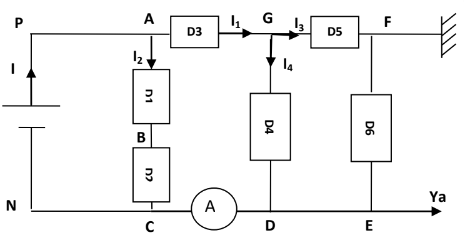
\includegraphics[width=0.42\textwidth]{./img/ex01.png}
	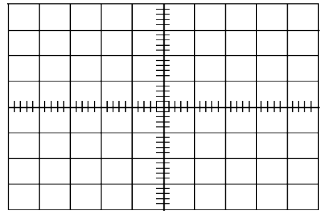
\includegraphics[width=0.32\textwidth]{./img/ex011.png}
\end{center}
On considère le circuit électrique représenté
ci-contre constitué de dipôles
électriques de D1 à D6. 

\textbf{On donne :}

\begin{itemize}
	\item \textbf{ $D_1$ et $D_2$ sont identiques.}

	\item $I = 9 mA$ ; $I_1 = 6 mA$ ; $I_4 = 2 mA$ ;
	\item $U_{PN} = 9V$ ; $U_{DG} = - 4 V$ ; $U_{FE} = 1 V$.
\end{itemize}

\begin{enumerate}
	\item Indiquer quelle tension l’oscilloscope mesure-t-il puis dessiner l'oscillogramme obtenu dans le cadre
ci-contre sachant que $S_V = 1 V / div$. \dotfill (1pt)
\item Déterminer le nombre de divisions indiqués par l’aiguille de l’ampèremètre sachant que le nombre de
divisions total est $100$ et le calibre choisi est $10 mA$.\dotfill (1pt)

\item Calculer les intensités de courant $I_2$ et $I_3$ en justifiant votre réponse.\dotfill(1pt)

\item calculer les tensions suivantes $U_{AG}$ ; $U_{AB}$ ; $U_{CB}$ ; $U_{FG}$ . justifier votre réponse. \dotfill(1pt)
\end{enumerate}



 \section*{Partie 2 :Montages électriques \dotfill(4 pts)}
Soit le circuit électrique suivant.
	\begin{center}
	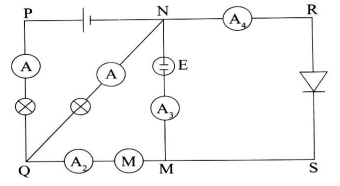
\includegraphics[width=0.45\textwidth]{./img/ex02.png}
\end{center}
\begin{enumerate}
	\item Reproduire le schéma et indiquer le sens du courant dans chaque branche
du circuit.\dotfill(1pt)

\item  Dans quel sens se déplacent les électrons dans la branche QM ?\dotfill(0,25pts)

\item On veut mesurer les intensités des courants dans ce circuit.
	\begin{enumerate}
		\item Compléter le tableau suivant par ce qui convient.\dotfill(0,75pts)
		
\begin{center}
\begin{tabular}{ | c | c | c | c| c| }
	\hline
	\textbf{Ampèremètre}& \textbf{Calibre} & \textbf{Lecture (n) div} & \textbf{cadron $n_0$ div}  & \textbf{Intensité}\\\hline 

	$A_1$ & 1A & 50 div& 100 div&$I_1$= ..... A \\\hline  
	$A_2$ & .... & 7 div& 30 div&$I_2$= 0,07 A \\\hline  
	$A_3$ & $100mA$ & 70 div& 100 div&$I_3$= ..... A \\\hline  
\end{tabular}
\end{center}


		\item Déterminer la quantité d’électricité Q qui traverse l’électrolyseur E pendant 20min.\dotfill(1pt)


		\item Déterminer les intensités manque $I$ et $I_4$ mesurées respectivement par les ampèremètres $A$ et $A_4$.\dotfill(1pt)

\end{enumerate}
\end{enumerate}


 \section*{Partie 3 :Court-circuit \dotfill(2 pts)}
Un élève a effectué le montage du circuit schématisé sur la
figure ci-contre.
	\begin{center}
	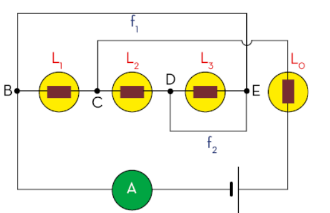
\includegraphics[width=0.45\textwidth]{./img/ex03.png}
\end{center}
Les quatre lampes sont identiques et f1 et f2 sont deux fils de
court-circuit.
L'ampèremètre A, indique la valeur 0,3 A.
\begin{enumerate}

\item Simplifier le schéma du montage.\dotfill(1pt)
\item  Calculer l'intensité du courant traversant chaque lampe.\dotfill(1pt)
\end{enumerate}
 \section*{Partie 4 :Utiliser un oscilloscope  \dotfill(3 pts)}
On considère le circuit représenté sur la figure ci-contre, et
qui est constitué de.
	\begin{center}
	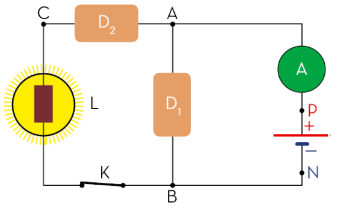
\includegraphics[width=0.45\textwidth]{./img/ex04.png}
\end{center}
\begin{itemize}
	\item  Un générateur maintenant entre ses borne une tension
constante UPN ;
\item Deux résistors $D_1$ et $D_2$ de résistances respectives $R_1$ et $R_2$ ;

\item Une lampe L ;
\item Un ampèremètre A et un voltmètre V
\item Un interrupteur K.
\item  L’interrupteur K étant fermé, l’ampèremètre et le voltmètre indiquent respectivement les valeurs $I$=$0,5 A$ et $U = 0,5 V $
\item Donnée : $R_2 = 3\Omega$ , $R_1 =15 \Omega$.
\end{itemize}

\begin{enumerate}

	\item L’interrupteur K étant fermé, Montrer que l’intensité $I_1$ du courant traversant le résistor $D_1$ peut s’écrire sous la forme : 
		$$I_1 = \frac{R_2.I + U}{R_1 + R_2}$$ .Calculer la valeur de $I_1$.\dotfill(1pt)
	\item Calculer la valeur de la tension $U_{PN}$.\dotfill(0,5pts)
	\item Déterminer $U_{CA}$ en fonction de $R_2$ et $U_{PN}$.\dotfill(0,5pts)
	\item La tension $U_{CA}$ est mesurée à l’aide d’un oscilloscope
utilisé avec la sensibilité verticale $S_V$=$0,5 V/div$. \\représenter sur la figure précédente le branchement de
l’oscilloscope.\dotfill(0,5pts)
\item représente l’écran de
l’oscilloscope. Représenter dessus le trait lumineux.\dotfill(0,5pts)
\end{enumerate}


\end{document}
